%%%%%%%%%%%%%%%%%%%%%%%%%%%%%%%%%%%%%%%%%%%%%%%%%%%%%%%%%%%%%%%%%%%%%%%%%%%%%
%% 
%% upated by @jhollist 09/15/2014
%% inspired by @cboetting https://github.com/cboettig/template and
%% @rmflight blog posts:
%% http://rmflight.github.io/posts/2014/07/analyses_as_packages.html 
%% http://rmflight.github.io/posts/2014/07/vignetteAnalysis.html).  
%%%%%%%%%%%%%%%%%%%%%%%%%%%%%%%%%%%%%%%%%%%%%%%%%%%%%%%%%%%%%%%%%%%%%%%%%%%%%
% Modifed from writeLaTex:
% Welcome to writeLaTeX --- just edit your LaTeX on the left,
% and we'll compile it for you on the right. If you give 
% someone the link to this page, they can edit at the same
% time. See the help menu above for more info. Enjoy!
%
%%%%%%%%%%%%%%%%%%%%%%%%%%%%%%%%%%%%%%%%%%%%%%%%%%%%%%%%%%%%%%%
%
% For more detailed article preparation guidelines, please see:
% http://f1000research.com/author-guidelines and http://f1000research.com/data-preparation

\documentclass[10pt,a4paper,twocolumn]{article}
\usepackage{components/f1000_styles}
\usepackage{longtable,booktabs}
\setcounter{secnumdepth}{0}
\begin{document}


\title{\textit{F1000Research} Example Manuscript: A template for using an R package to house a
reproducible manuscript}


\author[]{Jeffrey W. Hollister}

\affil[1]{}

\maketitle
\thispagestyle{fancy}


%%Adds affiliations from YAML

\begin{abstract}

Lorem ipsum dolor sit amet, consectetur adipiscing elit. Integer in sem sed sem pharetra eleifend vitae id massa. Curabitur et erat sit amet enim gravida dapibus quis vel ex. Maecenas luctus suscipit magna id vehicula. Quisque tincidunt auctor dignissim. Nunc vitae nulla vel lorem facilisis interdum non in mi. Donec fringilla luctus lacus ut egestas. Pellentesque eget tellus et ante tristique euismod. Proin at scelerisque ex, ac faucibus sem. In nec efficitur nulla. Nam libero augue, tristique et neque sed, pellentesque commodo lacus. Morbi vitae ultrices arcu. Suspendisse elit neque, placerat vitae venenatis id, auctor vestibulum augue. Vivamus iaculis magna at sapien sodales, a sagittis tellus sagittis. Sed laoreet ac massa id fringilla. In et enim eget ante tincidunt aliquet ut in risus. In vestibulum, nisl non viverra ullamcorper, odio nisl scelerisque sapien, vitae ornare neque odio ut odio. Maecenas vitae leo rhoncus, egestas quam ac, dapibus eros. Quisque molestie venenatis urna quis malesuada. Sed malesuada semper malesuada. Nulla aliquet maximus urna eu eleifend. Suspendisse elementum est vel ornare pulvinar. Curabitur quis aliquet massa, eget sollicitudin tellus. Phasellus tempus urna molestie finibus ultricies.

\end{abstract}

\section{Introduction}\label{introduction}

Nullam et accumsan urna, mollis vulputate dolor. Donec nec nisl
sagittis, laoreet nibh a, imperdiet eros. Ut sagittis ipsum diam. Nulla
auctor justo eu ante sodales sollicitudin. Aenean leo lacus, consequat
et aliquet vel, faucibus sit amet mi. Donec non nunc nec turpis cursus
mattis a vel eros. Sed sit amet velit lacinia, congue est non, pulvinar
dolor. Suspendisse felis erat, congue sit amet nunc nec, semper
porttitor magna. Nunc Hollister et al. (2011) eu ornare purus.
Suspendisse id nulla in massa pharetra fringilla. Quisque vestibulum
diam a ligula scelerisque, sit amet suscipit erat laoreet. Phasellus
erat turpis, porta at nisi nec, eleifend interdum sem.

Suspendisse elit neque, placerat vitae venenatis id, auctor vestibulum
augue. Vivamus iaculis magna at sapien sodales, a sagittis tellus
sagittis. Sed laoreet ac massa id fringilla. In et enim eget ante
tincidunt aliquet ut in risus. In vestibulum, nisl non viverra
ullamcorper, odio nisl scelerisque sapien, vitae ornare neque odio ut
odio. Maecenas vitae leo rhoncus, egestas quam ac, dapibus eros. Quisque
molestie venenatis urna quis malesuada. Sed malesuada semper malesuada.
Nulla aliquet maximus urna eu eleifend. Suspendisse elementum est vel
ornare pulvinar. Curabitur quis aliquet massa, eget sollicitudin tellus.
Phasellus tempus urna molestie finibus ultricies.

\section{Methods}\label{methods}

\subsection{Data and Study Area}\label{data-and-study-area}

Sed in augue non augue finibus lobortis. Maecenas imperdiet metus non
nisi imperdiet feugiat. Duis ac mauris metus. Nunc tempus est quis metus
consectetur, nec suscipit dui condimentum. Nam quis neque eu magna
suscipit imperdiet quis quis odio. Curabitur dignissim lorem eu risus
placerat fringilla. Fusce a odio eleifend neque semper sodales vitae eu
dui. Nullam laoreet, diam pellentesque gravida eleifend, lorem massa
sollicitudin tellus, et convallis nibh neque quis metus. Interdum et
malesuada fames ac ante ipsum primis in faucibus.

Nullam diam quam, egestas sed erat quis, placerat tincidunt nisl. Sed
varius ac tortor eget fermentum. Sed ac magna tellus. Cras dolor felis,
gravida eu lacus eget, convallis efficitur lacus. In vulputate neque
quis eros consectetur, sit amet vehicula quam consequat. Nulla euismod
quis lorem sit amet dapibus. Nam hendrerit ante et leo rutrum dignissim.
Maecenas semper nec magna quis aliquam. Vivamus urna purus, lobortis ut
imperdiet a, pretium in mauris.(Homer et al. 2004, USEPA 2009, Xian et
al. 2009, Hollister and Milstead 2010, Hollister et al. 2011, Beaulieu
et al. 2013, Hollister 2014).

Nullam et accumsan urna, mollis vulputate dolor. Donec nec nisl
sagittis, laoreet nibh a, imperdiet eros. Ut sagittis ipsum diam. Nulla
auctor justo eu ante sodales sollicitudin. Aenean leo lacus, consequat
et aliquet vel, faucibus sit amet mi. Donec non nunc nec turpis cursus
mattis a vel eros. Sed sit amet velit lacinia, congue est non, pulvinar
dolor. (USEPA 2009). Suspendisse felis erat, congue sit amet nunc nec,
semper porttitor magna. Nunc eu ornare purus. Suspendisse id nulla in
massa pharetra fringilla. Quisque vestibulum diam a ligula scelerisque,
sit amet suscipit erat laoreet. Phasellus erat turpis, porta at nisi
nec, eleifend interdum sem. (Homer et al. 2004, Xian et al. 2009).

Suspendisse elit neque, placerat vitae venenatis id, auctor vestibulum
augue. Vivamus iaculis magna at sapien sodales, a sagittis tellus
sagittis. Sed laoreet ac massa id fringilla. In et enim eget ante
tincidunt aliquet ut in risus(Table \ref{tab:Table1}). In vestibulum,
nisl non viverra ullamcorper, odio nisl scelerisque sapien, vitae ornare
neque odio ut odio. Maecenas vitae leo rhoncus, egestas quam ac, dapibus
eros.

\% latex table generated in R 3.1.1 by xtable 1.7-4 package \% Tue Oct
21 12:55:31 2014

\begin{table}[ht]
\centering
\begin{tabular}{rrrrrl}
  \hline
 & Sepal.Length & Sepal.Width & Petal.Length & Petal.Width & Species \\ 
  \hline
1 & 5.10 & 3.50 & 1.40 & 0.20 & setosa \\ 
  2 & 4.90 & 3.00 & 1.40 & 0.20 & setosa \\ 
  3 & 4.70 & 3.20 & 1.30 & 0.20 & setosa \\ 
  4 & 4.60 & 3.10 & 1.50 & 0.20 & setosa \\ 
  5 & 5.00 & 3.60 & 1.40 & 0.20 & setosa \\ 
  6 & 5.40 & 3.90 & 1.70 & 0.40 & setosa \\ 
   \hline
\end{tabular}
\end{table}

:This is the first example table\label{tab:Table1}

\section{Results}\label{results}

Nullam et accumsan urna, mollis vulputate dolor. Donec nec nisl
sagittis, laoreet nibh a, imperdiet eros. Ut sagittis ipsum diam. Nulla
auctor justo eu ante sodales sollicitudin. Aenean leo lacus, consequat
et aliquet vel, faucibus sit amet mi. Donec non nunc nec turpis cursus
mattis a vel eros. Sed sit amet velit lacinia, congue est non, pulvinar
dolor (Figure \ref{fig:Fig1}). Suspendisse felis erat, congue sit amet
nunc nec, semper porttitor magna (Table \ref{tab:Table2}). Nunc eu
ornare purus. Suspendisse id nulla in massa pharetra fringilla. Quisque
vestibulum diam a ligula scelerisque, sit amet suscipit erat laoreet.
Phasellus erat turpis, porta at nisi nec, eleifend interdum sem.

\begin{figure}[htbp]
\centering
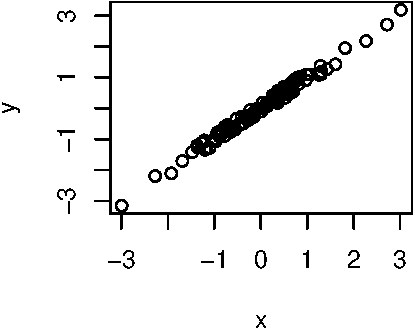
\includegraphics{./F1000Research_files/figure-latex/Fig1.pdf}
\caption{Just my first figure with a very fantastic
caption.\label{fig:Fig1}}
\end{figure}

\% latex table generated in R 3.1.1 by xtable 1.7-4 package \% Tue Oct
21 12:55:32 2014

\begin{table}[ht]
\centering
\begin{tabular}{rrrrrl}
  \hline
 & Sepal.Length & Sepal.Width & Petal.Length & Petal.Width & Species \\ 
  \hline
1 & 5.10 & 3.50 & 1.40 & 0.20 & setosa \\ 
  2 & 4.90 & 3.00 & 1.40 & 0.20 & setosa \\ 
  3 & 4.70 & 3.20 & 1.30 & 0.20 & setosa \\ 
  4 & 4.60 & 3.10 & 1.50 & 0.20 & setosa \\ 
  5 & 5.00 & 3.60 & 1.40 & 0.20 & setosa \\ 
  6 & 5.40 & 3.90 & 1.70 & 0.40 & setosa \\ 
   \hline
\end{tabular}
\end{table}

:A second table showing some of the mtcars dataset.\label{tab:Table2}

Nullam et accumsan urna, mollis vulputate dolor. Donec nec nisl
sagittis, laoreet nibh a, imperdiet eros. Ut sagittis ipsum diam. Nulla
auctor justo eu ante sodales sollicitudin. Aenean leo lacus, consequat
et aliquet vel, faucibus sit amet mi. Donec non nunc nec turpis cursus
mattis a vel eros. Sed sit amet velit lacinia, congue est non, pulvinar
dolor (Figure \ref{fig:Fig2}). Suspendisse felis erat, congue sit amet
nunc nec, semper porttitor magna. Nunc eu ornare purus. Suspendisse id
nulla in massa pharetra fringilla. Quisque vestibulum diam a ligula
scelerisque, sit amet suscipit erat laoreet. Phasellus erat turpis,
porta at nisi nec, eleifend interdum sem.

\begin{figure}[htbp]
\centering
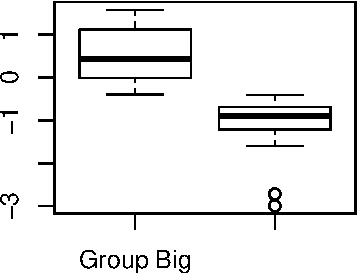
\includegraphics{./F1000Research_files/figure-latex/Fig2.pdf}
\caption{Second figure showing a boxplot with ground breaking results.
\label{fig:Fig2}}
\end{figure}

\section{Discussion}\label{discussion}

Lorem ipsum dolor sit amet, consectetur adipiscing elit. Integer in sem
sed sem pharetra eleifend vitae id massa. Curabitur et erat sit amet
enim gravida dapibus quis vel ex. Maecenas luctus suscipit magna id
vehicula. Quisque tincidunt auctor dignissim. Nunc vitae nulla vel lorem
facilisis interdum non in mi. Donec fringilla luctus lacus ut egestas.
Pellentesque eget tellus et ante tristique euismod. Proin at scelerisque
ex, ac faucibus sem. In nec efficitur nulla. Nam libero augue, tristique
et neque sed, pellentesque commodo lacus. Morbi vitae ultrices arcu.

Nullam et accumsan urna, mollis vulputate dolor. Donec nec nisl
sagittis, laoreet nibh a, imperdiet eros. Ut sagittis ipsum diam. Nulla
auctor justo eu ante sodales sollicitudin. Aenean leo lacus, consequat
et aliquet vel, faucibus sit amet mi. Donec non nunc nec turpis cursus
mattis a vel eros. Sed sit amet velit lacinia, congue est non, pulvinar
dolor. Suspendisse felis erat, congue sit amet nunc nec, semper
porttitor magna. Nunc eu ornare purus. Suspendisse id nulla in massa
pharetra fringilla. Quisque vestibulum diam a ligula scelerisque, sit
amet suscipit erat laoreet. Phasellus erat turpis, porta at nisi nec,
eleifend interdum sem.

Suspendisse elit neque, placerat vitae venenatis id, auctor vestibulum
augue. Vivamus iaculis magna at sapien sodales, a sagittis tellus
sagittis. Sed laoreet ac massa id fringilla. In et enim eget ante
tincidunt aliquet ut in risus. In vestibulum, nisl non viverra
ullamcorper, odio nisl scelerisque sapien, vitae ornare neque odio ut
odio. Maecenas vitae leo rhoncus, egestas quam ac, dapibus eros. Quisque
molestie venenatis urna quis malesuada. Sed malesuada semper malesuada.
Nulla aliquet maximus urna eu eleifend. Suspendisse elementum est vel
ornare pulvinar. Curabitur quis aliquet massa, eget sollicitudin tellus.
Phasellus tempus urna molestie finibus ultricies.

\section*{References}\label{references}
\addcontentsline{toc}{section}{References}

Beaulieu, M., F. Pick, and I. Gregory-Eaves. 2013. Nutrients and water
temperature are significant predictors of cyanobacterial biomass in a
1147 lakes data set. Limnol. Oceanogr 58:1736--1746.

Hollister, J. W. 2014. lakemorpho: Lake morphometry in r.

Hollister, J. W., W. B. Milstead, and M. A. Urrutia. 2011. Predicting
maximum lake depth from surrounding topography. PLoS ONE 6:e25764.

Hollister, J., and W. B. Milstead. 2010. Using gIS to estimate lake
volume from limited data. Lake and Reservoir Management 26:194--199.

Homer, C., C. Huang, L. Yang, B. Wylie, and M. Coan. 2004. Development
of a 2001 national land-cover database for the united states.
Photogrammetric Engineering \& Remote Sensing 70:829--840.

USEPA. 2009. National lakes assessment: a collaborative survey of the
nation's lakes. ePA 841-r-09-001. Office of Water; Office of Research;
Development, US Environmental Protection Agency Washington, DC.

Xian, G., C. Homer, and J. Fry. 2009. Updating the 2001 national land
cover database land cover classification to 2006 by using landsat
imagery change detection methods. Remote Sensing of Environment
113:1133--1147.

\nocite{*}
{\small\bibliographystyle{unsrt}
\bibliography{components/manuscript}}

\end{document}